\section{Discussion}
\label{sec:discussion}

The bounds are lower bounds on a resource, not a pulse-design prescription. Free and
exact $X$ rotations can rearrange how the systematic $Z$ error accumulates, but when the
common $Z$ scale is turned down to $\lambda=0$ every costly evolution disappears, and the
carrier must connect two separated endpoints while being extremely flat at $\lambda=1$.

\subsection{What the ladder rules out and the orders that matter}

At every order the cost is bounded below by the
elementary bound, hence by $4(N+1)/\mathrm{e}$: no arrangement of free rotations, however many,
makes high-order robustification sublinear. The exact-criterion rung gives $\cstar(\pi)\ge4$, while the sequences of
Ref.~\cite{Low2014} transcribed to this model cost $T=(2N+1)\pi$ and hence give
$\cstar(\pi)\le2\pi$; so
\begin{equation}
4\;\le\;\cstar(\pi)\;\le\;2\pi ,
\label{eq:window}
\end{equation}
an interval of width $2\pi-4\approx2.28$, whose endpoints differ by the factor $\pi/2$; the numerical costs of
Sec.~\ref{sec:numerics} are fitted by $T\approx5.26N+2.81$ for $N\le8$ and lie within a factor
$2.0$ of the reference line $4N$ at $N=1$ and within $1.4$ at $N=8$; the excess over $4N$ is
bounded in relative terms, so the remaining question is one of a constant factor rather than of
a new regime. Moreover, the model already grants the designer everything a fast-control layer could
offer---exact, instantaneous and free $X$ rotations in unlimited number and at arbitrary
positions, with the target reached exactly at the nominal error---and the bound is still linear:
here, a rich enough fast-control layer does not make the uncertain evolution asymptotically
efficient.

\paragraph{Why the idealization makes the bounds conservative.} The model is thin by design and every assumption favors the designer: one common multiplicative error, no time dependence, no decoherence, no leakage, instantaneous and perfect transverse control. Any model closer to a laboratory adds constraints, and adding constraints can only raise the least cost of an order-$N$ robust sequence.

\paragraph{Finite order, incoherent errors, and the orders that matter.} A device does
not get to choose $N$ freely: a longer sequence also spends more time in the presence of
decay, the tension that shapes time-optimal gate design on Rydberg platforms~\cite{Jandura2022}. Writing $\omega$ for the rate at which the uncertain $Z$-phase
accumulates and $\gamma$ for the decay rate, an order-$N$ sequence of cost $T$ pays an
incoherent infidelity of order $\gamma T/\omega$ while its coherent error falls like
$\eps^{N+1}$, and the two balance at
\begin{equation}
N^\ast\;\approx\;\frac{\ln(\omega/\gamma)}{2\ln(1/\eps)},
\label{eq:nstar}
\end{equation}
so the useful order grows only logarithmically as coherence improves. At the parameters of Fig.~\ref{fig:phys} the estimate gives $N^\ast\approx3.0$, up to the order-one prefactor of the coherent term; the tabulated sequences place the minimum at $N^\ast=2$.

This is where the
finite-order form of the bounds matters: the relevant orders are small, and there the
operative terms of~\eqref{eq:allN} are the elementary and Jensen rungs, which supply the cost side of
the balance at every order and without a threshold. The tradeoff
cannot be evaded by inventing better pulses, only by improving $\gamma$, $\eps$, or the
resource model itself. Figure~\ref{fig:phys} evaluates the balance at parameters
representative of current neutral-atom arrays: the optimum is at $N^\ast=2$, and improving
$\gamma/\omega$ by three orders of magnitude moves it only to $4$.

\begin{figure}[t]\centering
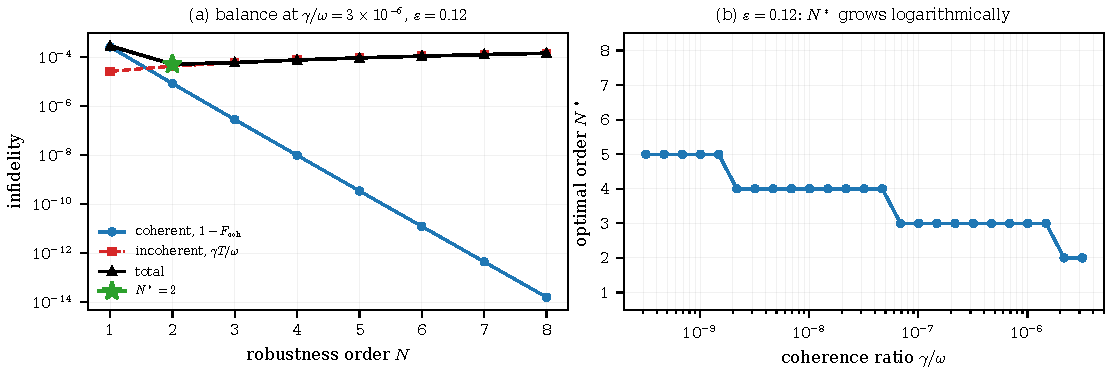
\includegraphics[width=0.93\linewidth]{figphys.pdf}
\caption{The coherent-versus-incoherent balance at parameters representative of current
neutral-atom arrays: interaction strengths $V/2\pi$ of a few hundred MHz at
few-micrometre separations~\cite{Evered2023,Mohan2023} and Rydberg lifetimes of order
$10^2\,\mu$s~\cite{Beterov2009}, which for $V/2\pi=500$~MHz and $\gamma/2\pi\approx1.6$~kHz
give a coherence ratio $\gamma/\omega\approx3\times10^{-6}$, together with a systematic
variation $\eps=0.12$. (a) Coherent
infidelity $\sin^2(\delta(\eps)/2)$ of the sequences of Table~\ref{tab:num}, the incoherent
infidelity $\gamma T/\omega$ they accumulate, and the sum; the minimum is at $N^\ast=2$. (b) The
same balance over four decades of the coherence ratio; the optimum moves only to $N^\ast=4$
after three decades and to $N^\ast=5$ after four. The
sequences plotted are those of Table~\ref{tab:num} with $N\le8$; both terms are evaluated on
those admissible sequences, so the plotted total is an upper bound on the infidelity achievable
at that order.}
\label{fig:phys}
\end{figure}

\subsection{Negatives: what cannot improve the ladder}

\paragraph{No third algebraic doubling.} The replacement method uses only two pieces of
information: the band $|\mu_m|\le\tauvar$ and the flatness $h^{(k)}(1)=0$, $k<q$, with
$q=2N+2$. The class of
replacements available to the method is $\Pi_{q-1}$: every polynomial of degree $<q$ qualifies,
and a continuous $Q$ that annihilates the twisted moment measures of every admissible sequence
lies in the uniform closure of $\Pi_{q-1}$ on $[-\tauvar,\tauvar]$, which is $\Pi_{q-1}$ itself
because that space is finite-dimensional and hence closed. The converse richness statement ---
that the admissible moment measures are weak-$*$ dense in the measures whose moments of order
$<q$ vanish --- is what would make the class exactly $\Pi_{q-1}$, and we do not prove it. Within
this class, no determinant, character identity, or higher trace power adds a functional. Moreover, products preserve the flatness-to-band ratio: if $h_1,h_2$ have
bands $\tauvar_1,\tauvar_2$ and flatness orders $q_1,q_2$ at $1$, then $h_1h_2$ has band
$\tauvar_1+\tauvar_2$ and flatness order $q_1+q_2$, so the threshold $\tauvar<q$ -- the
source of the coefficient~$4$ -- is unchanged by any power trick. The one explicit
square-root variant is strictly worse because it halves the order: writing
$V_\lambda=U_1^\dagger U_\lambda=a+\mathrm{i}\mathbf{b}\cdot\bm{\sigma}$ gives
$h=|\mathbf{b}|^2/(1+a)$, where each component $b_j$ has band $\tauvar$ but flatness only
$N+1$, so that route needs $\tauvar\lesssim N+1$, i.e.\ asymptotic coefficient~$2$. There
is no third doubling of the coefficient, only a reparametrisation.

\paragraph{The minimax polynomial is marginal.} Let $E_{q-1}(\tauvar)$ be the best uniform
approximation error of $\mathrm{e}^{-\mathrm{i}\mu}$ on $[-\tauvar,\tauvar]$ by degree-$<q$ polynomials, and
let $\varepsilon^{\mathrm{tr}}$ be the Chebyshev-truncation error used by the rung. The
$L^2$ argument with the Chebyshev probability weight gives
$\sqrt2\,|c_q|\le E_{q-1}(\tauvar)\le\varepsilon^{\mathrm{tr}}\le2\sum_{k\ge q}|c_k|$,
so replacing the truncation by the optimal polynomial improves the error by at most a
constant factor. Since the rung criterion is a condition on the error at the log level, a
constant factor shifts the exponent by an additive constant only, and the asymptotic
coefficient stays~$4$.
\begin{remark}[Numeric illustration, not a theorem]
Relaxing the error threshold by a factor $F=2$ moves the largest admissible $\tauvar$ at
$N=12$ from $14.176$ to $14.581$, an increase of about $+2.9\%$; larger relaxations add a few
further percent. These are computed illustrations
only: the minimax direction is a refinement, never a new rung.
\end{remark}

\paragraph{The free $X$-angle gives nothing at $\phi=\pi$.} The exact endpoint identity
is $h(0)=1-\cos(\phi/2)\cos(A/2)$ with $A=\sum_j\alpha_j$ free. At $\phi=\pi$ one has
$\cos(\phi/2)=0$, so $h(0)=1$ for every $A$: no parity, topological, or other constraint
on $A$ can improve the endpoint bound in the worst case, which is the case the theorem is
about. At $\phi<\pi$, $\min_Ah(0)=1-\cos(\phi/2)=2\sin^2(\phi/4)$, attained at
$A\equiv\pi$, which is exactly the bound used here. The genuinely larger endpoint
constant $|\mathbf{b}(0)|\ge\sin(\phi/2)$ belongs to the halved-order $\mathbf{b}$-vector
route above, which is asymptotically worse (its coefficient is $2$, not $4$), although at small
$\phi$ and small $N$ its larger endpoint constant can make it the stronger of the two.

\subsection{Ceiling: the dichotomy at $4$ and the open gap}
\label{sec:ceiling}

Can any argument using only the band data (band $\tauvar$, flatness order $q=2N+2$ at
$\lambda=1$, $\|h\|_\infty\le2$, endpoint $h(0)\ge2\sin^2(\phi/4)$) certify
$\liminf T/N>4$? The answer is equivalent to one exact obstruction. Call $\mathrm{UP}(q)$
the statement that there is a compactly supported density on $[-q,q]$ whose Fourier transform,
while maximal at the origin, is as small as $2^{-q}$ times that maximum at $O(1)$ distances
from it---equivalently, that the four band-data constraints at bandwidth $q$ are consistent
with an endpoint value $|h(0)|>1$. Two implications fix the status of the ceiling. If
$\mathrm{UP}(q)$ holds for every $q$, then no band-data argument certifies a coefficient
larger than $4$: a witness at bandwidth $q=2N+2$ satisfies every hypothesis used at order
$N$ while realizing $T=2q\approx4N$, so no argument built from those hypotheses can exclude
it. Conversely, if $\mathrm{UP}(q)$ fails for every sufficiently large $q$, then the band data
certify a coefficient larger than $4$: at each such order the four constraints already exclude
the corresponding bandwidth, so an argument passing $4$ exists. Whether the ceiling at $4$ holds
is thus decided exactly when this uncertainty principle is decided for all large $q$, and this
paper takes no position on it.

The ceiling at $4$ is \emph{open}. What is proved is the diagnosis on both sides. Every
natural candidate witness family fails $\mathrm{UP}(q)$ by the same quantitative
mechanism -- edge diffraction amplified by $|\cdot|^q$: sine powers give the $2\pi$
witness below but fail at $4$; polynomial bumps, Gaussians with any cutoff width, and
lattice profiles all fail with the endpoint-to-supremum ratio decaying exponentially in
$q$. Nor is $\mathrm{UP}(q)$ cheap to refute: no elementary argument eliminates it. What is
known unconditionally is threefold, and only the first of the three is proved in this paper:
the rung with coefficient $4$ (Theorem~\ref{thm:newrung}); a cap at $2\pi$ for every route
that uses the band data through the replacement mechanism, argued here as follows --- such a
route needs the best uniform approximation error $\varepsilon_q(\tauvar)$ of
$\mathrm{e}^{-\mathrm{i}\mu}$ on $[-\tauvar,\tauvar]$ by degree-$<q$ polynomials to fall below
$s/2\le1/2$, whereas $\varepsilon_q(\tauvar)\ge1$ once $\tauvar\ge\pi q/2$ (if
$|\mathrm{e}^{-\mathrm{i}\mu}-P|\le\varepsilon$ then $|\cos\mu-\Ree P|\le\varepsilon$;
$\cos$ alternates between $\pm1$ at $k\pi$, so for $\tauvar\ge\pi q/2$ there are more than
$q$ such points and Rolle forces $\Ree P$ to be constant, whence
$\varepsilon\ge1$), with the extremal witness $g(x)=2\sin^q(\pi x/2)$ of type $\pi q/2$
attaining the endpoint $2$; and the necessity that any admissible kernel have $L^1$ norm at
least the best-approximation error, which is the mechanism behind Theorem~\ref{thm:newrung}
and is machine-checked as \lean{realize_L1}. The $2\pi$ argument is a sketch in the sense
that it bounds the mechanism of Secs.~\ref{sec:newrung} and not every conceivable band-data
route. Thus $[4,2\pi]$ is the exact open gap for band-data
methods, sharp at the upper end by the sequence of Ref.~\cite{Low2014}, and this paper takes no position
on whether the ceiling at $4$ holds or fails.

\paragraph{Thresholds and numerics.} The closed-form threshold of~\eqref{eq:closedform} is
a sufficient condition assembled from explicit majorants -- a contour-shift coefficient
bound, a geometric tail sum, and kernel bookkeeping. The constant $6$ and the threshold
$500+\lceil\exp((11+|\log s_0|)/1.2)\rceil$ are conservative bookkeeping rather than
features of the control problem. The criterion~\eqref{eq:thm-newrung} being unverified
below a certified bandwidth is therefore not evidence that the coefficient is smaller
there; those orders are covered by the elementary and Jensen rungs.


\subsection{Conclusions}

The cost of cancelling a common systematic error to order $N$ in the free-$X$ model is
linear in $N$, and the four rungs of this paper pin down how much of the coefficient is
accessible to successively stronger arguments: $2/\e$ and $4/\e$ from one Taylor step,
$2\pi/\e$ once the carrier is treated as an entire function of exponential type, and a
coefficient approaching $4$ once its whole band is used. What is proved is therefore both a
statement about the resource and a statement about the method. On the resource side the
coefficient is linear in $N$ and confined to $[4,2\pi]$; on the method side, whether any
argument that uses only the bandwidth, the flatness order, the supremum bound and the endpoint
separation can pass $4$ is equivalent to the uncertainty principle $\mathrm{UP}(q)$ of
Sec.~\ref{sec:ceiling}; the cap at $2\pi$ for the mechanism used here is unconditional. At the small orders
that a device with realistic coherence actually uses the elementary and Jensen rungs already
supply the operative bound. The numerical sequences show that that sequence is not
optimal at any order considered, so the upper end is not rigid either. Extending any of these
statements---to non-common errors, to a full account of decoherence, or to a proof that the
ceiling at $4$ is attained or violated---would move the window, not the ladder.
